\begin{figure}[ht]
\centering
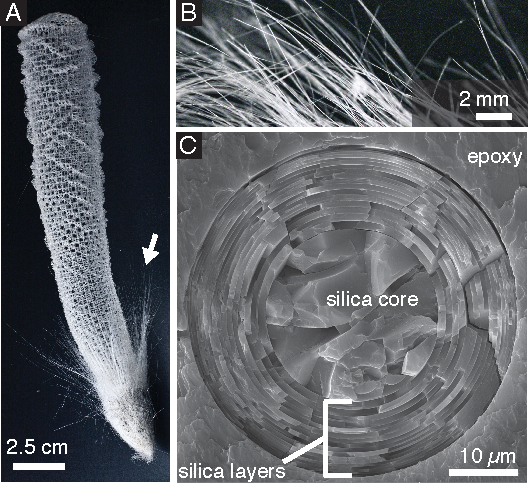
\includegraphics[width=0.7\textwidth]{Figures/Figure1_V5.pdf}
\caption{Structure of \textit{Euplectella aspergillum} (\EA) sponge. (\textsf{A}) An \EA skeleton (reprinted from~\cite{monn2015new}). The basalia spicules are identified with a white arrow. (\textsf{B}) A magnified view of the basalia spicules. (\textsf{C}) An SEM image of a cross-section of an \EA  spicule revealing its cylindrically layered architecture (modified from~\cite{monn2015new}).}
\label{fig:eastructure}
\end{figure}
